\lesson{17 Sep 2024}{Light-weight context}

\begin{definition}[Light-weight context]
A light-weight context (\textit{lwC}) is an OS abstraction that provides \textcolor{gray}{independent} units of isolation, privilege, and execution state \textbf{within} the process abstraction.
\end{definition}

\textit{lwC}s are motivated as follows:

\begin{itemize}
    \item \textcolor{gray}{Kernel} threads provide execution state (a.k.a. context) separation but lacks isolation support for other process states, e.g., memory, file descriptors, credentials, etc.
    \item Processes provide such isolation, but \verb|fork| syscall is expensive
\end{itemize}

\textit{lwC} interface is:

\begin{figure}[H]
\centering
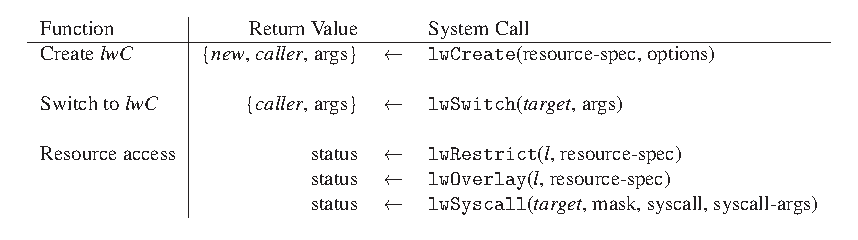
\includegraphics[width=1\linewidth]{figures/lwC_ifc.eps}
\end{figure}

A process starts with a root \textit{lwC}, and may create more \textit{lwC}s using \verb|lwCreate|, which inherits process \verb|fork| (or \verb|clone|) semantics. A \textit{lwC} is referenced by a \textit{descriptor}. It is destroyed when no more referenced. Parent \textit{lwC} have full control over shared resource with a child by passing the \verb|resource-spec| argument. \\

There can be multiple threads in a \textit{lwC}, and a thread may run in distinct \textit{lwC}s by calling \verb|lwSwitch|. \verb|lwSwitch| is similar to coroutine \verb|yield|.

\begin{note}
\textit{lwC}s are \textbf{not} schedulable and are orthogonal to kernel threads.
\end{note}

Resources can be mapped from a \textit{lwC} to another via \verb|lwOverlay|.

\subsection{Common \textit{lwC} use cases}

\begin{example}
Snapshot and rollback \\

Parent \textit{lwC} creates a child for a snapshot. Switch to this child \textit{lwC} to roll back program state.
\end{example}

\begin{example}
Isolation in event-driven design \\

Each client maps to a \textit{socket} on a server. Use distinct \textit{lwC}s for every socket. In this way, there will be no sensitive information leak between different sessions.
\end{example}

\begin{example}
Sensitive data isolation \\

Parent \textit{lwC} creates a child with full access to credentials. While parent relinquishes its own access, the child enters a loop to process, e.g., signature requests from a buffer.
\end{example}

\begin{example}
Protected reference monitor \\

Error code and signal are pass among \textit{lwC}s. Syscalls are monitored via \verb|lwSyscall|.
\end{example}

\textit{lwC}s have lower overhead than both kernel thread and process.
